\documentclass[twoside]{book}

% Packages required by doxygen
\usepackage{fixltx2e}
\usepackage{calc}
\usepackage{doxygen}
\usepackage[export]{adjustbox} % also loads graphicx
\usepackage{graphicx}
\usepackage[utf8]{inputenc}
\usepackage{makeidx}
\usepackage{multicol}
\usepackage{multirow}
\PassOptionsToPackage{warn}{textcomp}
\usepackage{textcomp}
\usepackage[nointegrals]{wasysym}
\usepackage[table]{xcolor}

% Font selection
\usepackage[T1]{fontenc}
\usepackage[scaled=.90]{helvet}
\usepackage{courier}
\usepackage{amssymb}
\usepackage{sectsty}
\renewcommand{\familydefault}{\sfdefault}
\allsectionsfont{%
  \fontseries{bc}\selectfont%
  \color{darkgray}%
}
\renewcommand{\DoxyLabelFont}{%
  \fontseries{bc}\selectfont%
  \color{darkgray}%
}
\newcommand{\+}{\discretionary{\mbox{\scriptsize$\hookleftarrow$}}{}{}}

% Page & text layout
\usepackage{geometry}
\geometry{%
  a4paper,%
  top=2.5cm,%
  bottom=2.5cm,%
  left=2.5cm,%
  right=2.5cm%
}
\tolerance=750
\hfuzz=15pt
\hbadness=750
\setlength{\emergencystretch}{15pt}
\setlength{\parindent}{0cm}
\setlength{\parskip}{3ex plus 2ex minus 2ex}
\makeatletter
\renewcommand{\paragraph}{%
  \@startsection{paragraph}{4}{0ex}{-1.0ex}{1.0ex}{%
    \normalfont\normalsize\bfseries\SS@parafont%
  }%
}
\renewcommand{\subparagraph}{%
  \@startsection{subparagraph}{5}{0ex}{-1.0ex}{1.0ex}{%
    \normalfont\normalsize\bfseries\SS@subparafont%
  }%
}
\makeatother

% Headers & footers
\usepackage{fancyhdr}
\pagestyle{fancyplain}
\fancyhead[LE]{\fancyplain{}{\bfseries\thepage}}
\fancyhead[CE]{\fancyplain{}{}}
\fancyhead[RE]{\fancyplain{}{\bfseries\leftmark}}
\fancyhead[LO]{\fancyplain{}{\bfseries\rightmark}}
\fancyhead[CO]{\fancyplain{}{}}
\fancyhead[RO]{\fancyplain{}{\bfseries\thepage}}
\fancyfoot[LE]{\fancyplain{}{}}
\fancyfoot[CE]{\fancyplain{}{}}
\fancyfoot[RE]{\fancyplain{}{\bfseries\scriptsize Generated by Doxygen }}
\fancyfoot[LO]{\fancyplain{}{\bfseries\scriptsize Generated by Doxygen }}
\fancyfoot[CO]{\fancyplain{}{}}
\fancyfoot[RO]{\fancyplain{}{}}
\renewcommand{\footrulewidth}{0.4pt}
\renewcommand{\chaptermark}[1]{%
  \markboth{#1}{}%
}
\renewcommand{\sectionmark}[1]{%
  \markright{\thesection\ #1}%
}

% Indices & bibliography
\usepackage{natbib}
\usepackage[titles]{tocloft}
\setcounter{tocdepth}{3}
\setcounter{secnumdepth}{5}
\makeindex

% Hyperlinks (required, but should be loaded last)
\usepackage{ifpdf}
\ifpdf
  \usepackage[pdftex,pagebackref=true]{hyperref}
\else
  \usepackage[ps2pdf,pagebackref=true]{hyperref}
\fi
\hypersetup{%
  colorlinks=true,%
  linkcolor=blue,%
  citecolor=blue,%
  unicode%
}

% Custom commands
\newcommand{\clearemptydoublepage}{%
  \newpage{\pagestyle{empty}\cleardoublepage}%
}

\usepackage{caption}
\captionsetup{labelsep=space,justification=centering,font={bf},singlelinecheck=off,skip=4pt,position=top}

%===== C O N T E N T S =====

\begin{document}

% Titlepage & ToC
\hypersetup{pageanchor=false,
             bookmarksnumbered=true,
             pdfencoding=unicode
            }
\pagenumbering{roman}
\begin{titlepage}
\vspace*{7cm}
\begin{center}%
{\Large My Project }\\
\vspace*{1cm}
{\large Generated by Doxygen 1.8.11}\\
\end{center}
\end{titlepage}
\clearemptydoublepage
\tableofcontents
\clearemptydoublepage
\pagenumbering{arabic}
\hypersetup{pageanchor=true}

%--- Begin generated contents ---
\chapter{Hierarchical Index}
\section{Class Hierarchy}
This inheritance list is sorted roughly, but not completely, alphabetically\+:\begin{DoxyCompactList}
\item \contentsline{section}{Cell}{\pageref{class_cell}}{}
\begin{DoxyCompactList}
\item \contentsline{section}{Hexahedron}{\pageref{class_hexahedron}}{}
\item \contentsline{section}{Pyramid}{\pageref{class_pyramid}}{}
\item \contentsline{section}{Tetrahedron}{\pageref{class_tetrahedron}}{}
\end{DoxyCompactList}
\item \contentsline{section}{cell\+Info}{\pageref{structcell_info}}{}
\item \contentsline{section}{Material}{\pageref{class_material}}{}
\item \contentsline{section}{Matrix3x3}{\pageref{class_matrix3x3}}{}
\item \contentsline{section}{Model}{\pageref{class_model}}{}
\item Q\+Dialog\begin{DoxyCompactList}
\item \contentsline{section}{App\+Help}{\pageref{class_app_help}}{}
\item \contentsline{section}{New\+Shape\+Choice}{\pageref{class_new_shape_choice}}{}
\end{DoxyCompactList}
\item Q\+Main\+Window\begin{DoxyCompactList}
\item \contentsline{section}{Main\+Window}{\pageref{class_main_window}}{}
\end{DoxyCompactList}
\item \contentsline{section}{Vector3D}{\pageref{class_vector3_d}}{}
\end{DoxyCompactList}

\chapter{Class Index}
\section{Class List}
Here are the classes, structs, unions and interfaces with brief descriptions\+:\begin{DoxyCompactList}
\item\contentsline{section}{\hyperlink{class_app_help}{App\+Help} }{\pageref{class_app_help}}{}
\item\contentsline{section}{\hyperlink{class_cell}{Cell} }{\pageref{class_cell}}{}
\item\contentsline{section}{\hyperlink{structcell_info}{cell\+Info} }{\pageref{structcell_info}}{}
\item\contentsline{section}{\hyperlink{class_hexahedron}{Hexahedron} }{\pageref{class_hexahedron}}{}
\item\contentsline{section}{\hyperlink{class_main_window}{Main\+Window} }{\pageref{class_main_window}}{}
\item\contentsline{section}{\hyperlink{class_material}{Material} }{\pageref{class_material}}{}
\item\contentsline{section}{\hyperlink{class_matrix3x3}{Matrix3x3} }{\pageref{class_matrix3x3}}{}
\item\contentsline{section}{\hyperlink{class_model}{Model} }{\pageref{class_model}}{}
\item\contentsline{section}{\hyperlink{class_new_shape_choice}{New\+Shape\+Choice} }{\pageref{class_new_shape_choice}}{}
\item\contentsline{section}{\hyperlink{class_pyramid}{Pyramid} }{\pageref{class_pyramid}}{}
\item\contentsline{section}{\hyperlink{class_tetrahedron}{Tetrahedron} }{\pageref{class_tetrahedron}}{}
\item\contentsline{section}{\hyperlink{class_vector3_d}{Vector3D} }{\pageref{class_vector3_d}}{}
\end{DoxyCompactList}

\chapter{Class Documentation}
\hypertarget{class_app_help}{}\section{App\+Help Class Reference}
\label{class_app_help}\index{App\+Help@{App\+Help}}
Inheritance diagram for App\+Help\+:\begin{figure}[H]
\begin{center}
\leavevmode
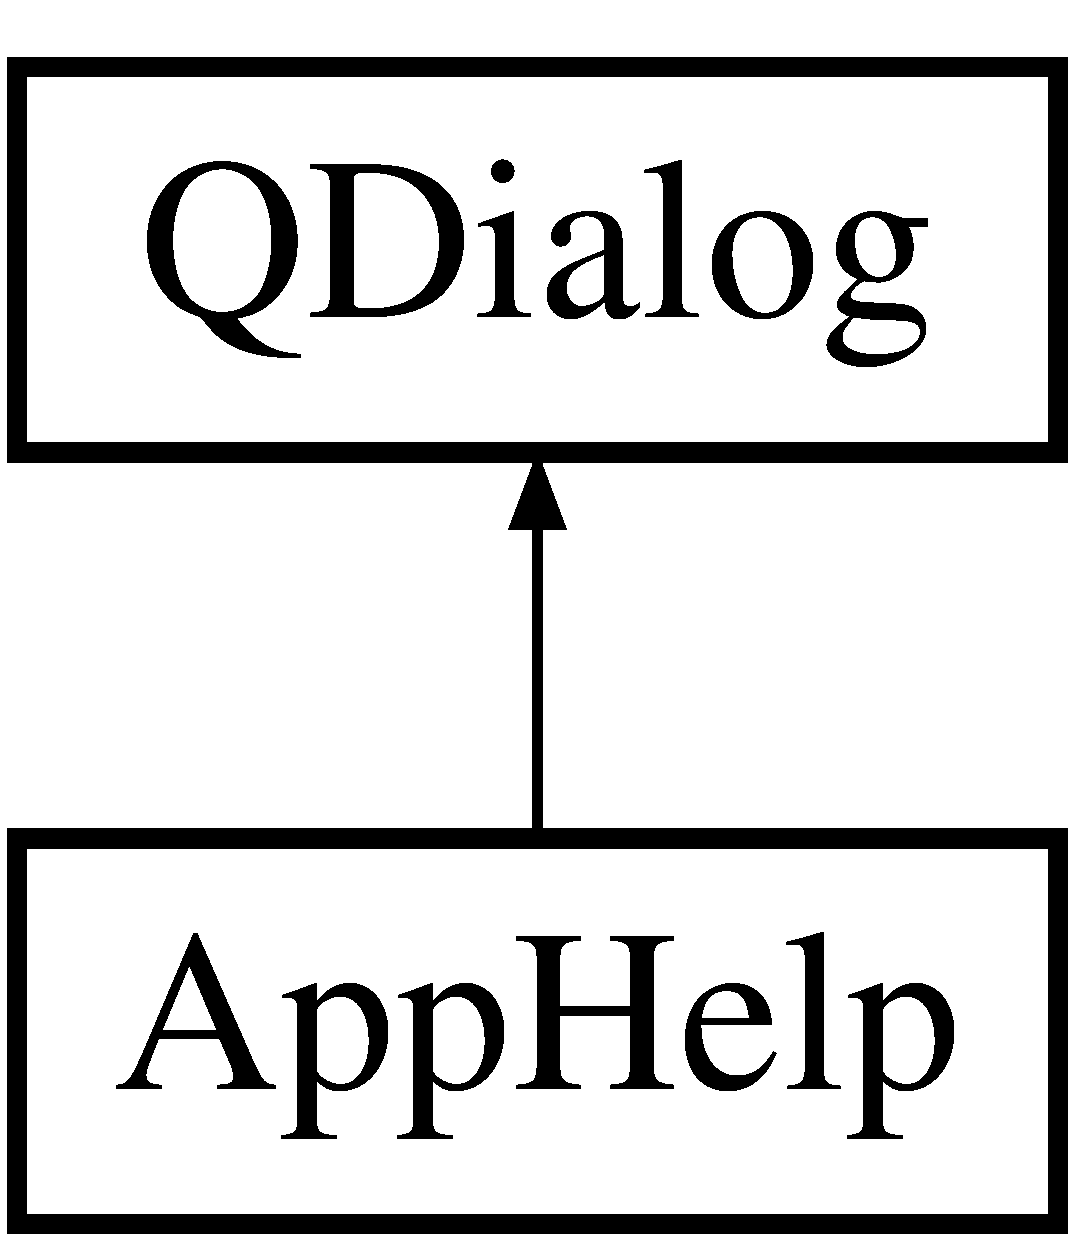
\includegraphics[height=2.000000cm]{class_app_help}
\end{center}
\end{figure}
\subsection*{Public Member Functions}
\begin{DoxyCompactItemize}
\item 
{\bfseries App\+Help} (Q\+Widget $\ast$parent=nullptr)\hypertarget{class_app_help_af11afe5130000748562f2a49a66d869b}{}\label{class_app_help_af11afe5130000748562f2a49a66d869b}

\item 
bool {\bfseries run\+Help} ()\hypertarget{class_app_help_af13259ffa31f8f85a1ea881e713bfc77}{}\label{class_app_help_af13259ffa31f8f85a1ea881e713bfc77}

\end{DoxyCompactItemize}


The documentation for this class was generated from the following files\+:\begin{DoxyCompactItemize}
\item 
/home/travis/build/\+Te\+Fka/2020\+\_\+\+G\+R\+O\+U\+P\+\_\+19/\+G\+U\+I\+\_\+source/apphelp.\+h\item 
/home/travis/build/\+Te\+Fka/2020\+\_\+\+G\+R\+O\+U\+P\+\_\+19/\+G\+U\+I\+\_\+source/apphelp.\+cpp\end{DoxyCompactItemize}

\hypertarget{class_cell}{}\section{Cell Class Reference}
\label{class_cell}\index{Cell@{Cell}}
Inheritance diagram for Cell\+:\begin{figure}[H]
\begin{center}
\leavevmode
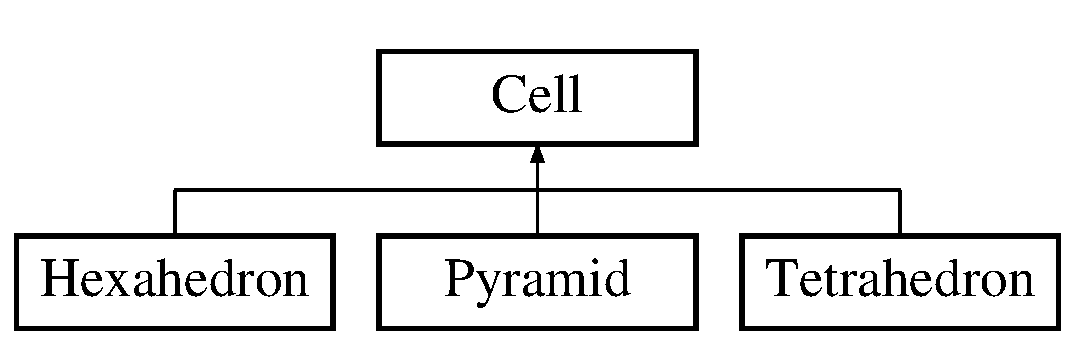
\includegraphics[height=2.000000cm]{class_cell}
\end{center}
\end{figure}
\subsection*{Public Member Functions}
\begin{DoxyCompactItemize}
\item 
{\bfseries Cell} (int, int, int, std\+::vector$<$ int $>$)\hypertarget{class_cell_ac2b3777a18c004d3ac03becf241259ca}{}\label{class_cell_ac2b3777a18c004d3ac03becf241259ca}

\item 
{\bfseries Cell} (const \hyperlink{class_cell}{Cell} \&)\hypertarget{class_cell_a8ca000885181236a713963c5c8bdb46f}{}\label{class_cell_a8ca000885181236a713963c5c8bdb46f}

\item 
int {\bfseries get\+ID} ()\hypertarget{class_cell_a6fb5e28360b3a6e53400af8b950f6203}{}\label{class_cell_a6fb5e28360b3a6e53400af8b950f6203}

\item 
int {\bfseries get\+Type} ()\hypertarget{class_cell_add3277569149cf78bb6a6e110eb119a6}{}\label{class_cell_add3277569149cf78bb6a6e110eb119a6}

\item 
int {\bfseries get\+Material\+ID} ()\hypertarget{class_cell_a7de149edc6b03f6e25ac75cb2b83709d}{}\label{class_cell_a7de149edc6b03f6e25ac75cb2b83709d}

\item 
std\+::vector$<$ int $>$ {\bfseries get\+Indices} ()\hypertarget{class_cell_abed068e37a2dc9d1972d3a5577429b0d}{}\label{class_cell_abed068e37a2dc9d1972d3a5577429b0d}

\item 
\hyperlink{class_vector3_d}{Vector3D} {\bfseries get\+Centre\+Of\+Gravity} ()\hypertarget{class_cell_ac6f89d89f65ac570dbfee6630e8ac77a}{}\label{class_cell_ac6f89d89f65ac570dbfee6630e8ac77a}

\item 
double {\bfseries get\+Weight} ()\hypertarget{class_cell_a8894ea0d3bf52c4837b95b7ec547392b}{}\label{class_cell_a8894ea0d3bf52c4837b95b7ec547392b}

\item 
double {\bfseries get\+Volume} ()\hypertarget{class_cell_aac8a5f3d06691efa17d909cc4e9c248b}{}\label{class_cell_aac8a5f3d06691efa17d909cc4e9c248b}

\item 
void {\bfseries set\+ID} (int)\hypertarget{class_cell_a8bb0817022a7e100b204ef7ba40d2789}{}\label{class_cell_a8bb0817022a7e100b204ef7ba40d2789}

\item 
void {\bfseries set\+Type} (int)\hypertarget{class_cell_a6dc5008f3f6d93dc0154ca62ec280771}{}\label{class_cell_a6dc5008f3f6d93dc0154ca62ec280771}

\item 
void {\bfseries set\+Material\+ID} (int)\hypertarget{class_cell_aff698048fe244dce00acf341428b5d12}{}\label{class_cell_aff698048fe244dce00acf341428b5d12}

\item 
void {\bfseries set\+Indices} (std\+::vector$<$ int $>$)\hypertarget{class_cell_a9af52dac7c4d4f01791fd0ad5f7b8125}{}\label{class_cell_a9af52dac7c4d4f01791fd0ad5f7b8125}

\item 
void {\bfseries push\+Indice} (int)\hypertarget{class_cell_a93dd64907a9608f6131e1042dfef16d1}{}\label{class_cell_a93dd64907a9608f6131e1042dfef16d1}

\item 
void {\bfseries insert\+Indice} (int, int)\hypertarget{class_cell_a569d618040b18f6b80bcc74ac2d155c2}{}\label{class_cell_a569d618040b18f6b80bcc74ac2d155c2}

\item 
void {\bfseries set\+Indice} (int, int)\hypertarget{class_cell_ab32d149f16f70270f01762ee79f0712c}{}\label{class_cell_ab32d149f16f70270f01762ee79f0712c}

\item 
void {\bfseries calc\+Weight} (std\+::vector$<$ \hyperlink{class_material}{Material} $>$)\hypertarget{class_cell_af458a98ed21d80438afac6a10f26f13c}{}\label{class_cell_af458a98ed21d80438afac6a10f26f13c}

\item 
void {\bfseries calc\+Centre\+Of\+Gravity} (std\+::vector$<$ \hyperlink{class_vector3_d}{Vector3D} $>$)\hypertarget{class_cell_a33ee01b65c3615852f0fb9f4d9d95d13}{}\label{class_cell_a33ee01b65c3615852f0fb9f4d9d95d13}

\end{DoxyCompactItemize}
\subsection*{Protected Attributes}
\begin{DoxyCompactItemize}
\item 
int {\bfseries ID}\hypertarget{class_cell_a94f1fa1e227b638d8732524e43589392}{}\label{class_cell_a94f1fa1e227b638d8732524e43589392}

\item 
int {\bfseries type}\hypertarget{class_cell_a6a3f3ec6c13524695884f3a302b23d88}{}\label{class_cell_a6a3f3ec6c13524695884f3a302b23d88}

\item 
int {\bfseries material\+ID}\hypertarget{class_cell_a7a478d78dd2f456cdcbdaa62c9a45323}{}\label{class_cell_a7a478d78dd2f456cdcbdaa62c9a45323}

\item 
double {\bfseries weight}\hypertarget{class_cell_a33f783e27040648251570bb281d5c744}{}\label{class_cell_a33f783e27040648251570bb281d5c744}

\item 
double {\bfseries volume}\hypertarget{class_cell_a426862431a79984cb040c6f396a8e1d9}{}\label{class_cell_a426862431a79984cb040c6f396a8e1d9}

\item 
\hyperlink{class_vector3_d}{Vector3D} {\bfseries centre\+\_\+of\+\_\+gravity}\hypertarget{class_cell_ab57b28c71b2dc2dcc7c95ac73b5b5375}{}\label{class_cell_ab57b28c71b2dc2dcc7c95ac73b5b5375}

\item 
std\+::vector$<$ int $>$ {\bfseries indices}\hypertarget{class_cell_a9e0ea8c2547718c8b34694d6d0db2c9e}{}\label{class_cell_a9e0ea8c2547718c8b34694d6d0db2c9e}

\end{DoxyCompactItemize}


The documentation for this class was generated from the following files\+:\begin{DoxyCompactItemize}
\item 
/home/travis/build/\+Te\+Fka/2020\+\_\+\+G\+R\+O\+U\+P\+\_\+19/\+Inc/Cell.\+h\item 
/home/travis/build/\+Te\+Fka/2020\+\_\+\+G\+R\+O\+U\+P\+\_\+19/\+Src/Cell.\+cpp\end{DoxyCompactItemize}

\hypertarget{structcell_info}{}\section{cell\+Info Struct Reference}
\label{structcell_info}\index{cell\+Info@{cell\+Info}}
\subsection*{Public Attributes}
\begin{DoxyCompactItemize}
\item 
int {\bfseries ID}\hypertarget{structcell_info_ab1aa474e08f44d86083037c014ad4746}{}\label{structcell_info_ab1aa474e08f44d86083037c014ad4746}

\item 
int {\bfseries material\+ID}\hypertarget{structcell_info_af226971bcc6ed0aa5a676623bb0b9c33}{}\label{structcell_info_af226971bcc6ed0aa5a676623bb0b9c33}

\item 
int {\bfseries type}\hypertarget{structcell_info_a62d34f940eb373d0f1657caea79d3e85}{}\label{structcell_info_a62d34f940eb373d0f1657caea79d3e85}

\item 
std\+::vector$<$ int $>$ {\bfseries indixes}\hypertarget{structcell_info_ab28d2d23ee7f5667488609a16b7a7084}{}\label{structcell_info_ab28d2d23ee7f5667488609a16b7a7084}

\end{DoxyCompactItemize}


The documentation for this struct was generated from the following file\+:\begin{DoxyCompactItemize}
\item 
/home/travis/build/\+Te\+Fka/2020\+\_\+\+G\+R\+O\+U\+P\+\_\+19/\+Inc/Model.\+h\end{DoxyCompactItemize}

\hypertarget{class_hexahedron}{}\section{Hexahedron Class Reference}
\label{class_hexahedron}\index{Hexahedron@{Hexahedron}}
Inheritance diagram for Hexahedron\+:\begin{figure}[H]
\begin{center}
\leavevmode
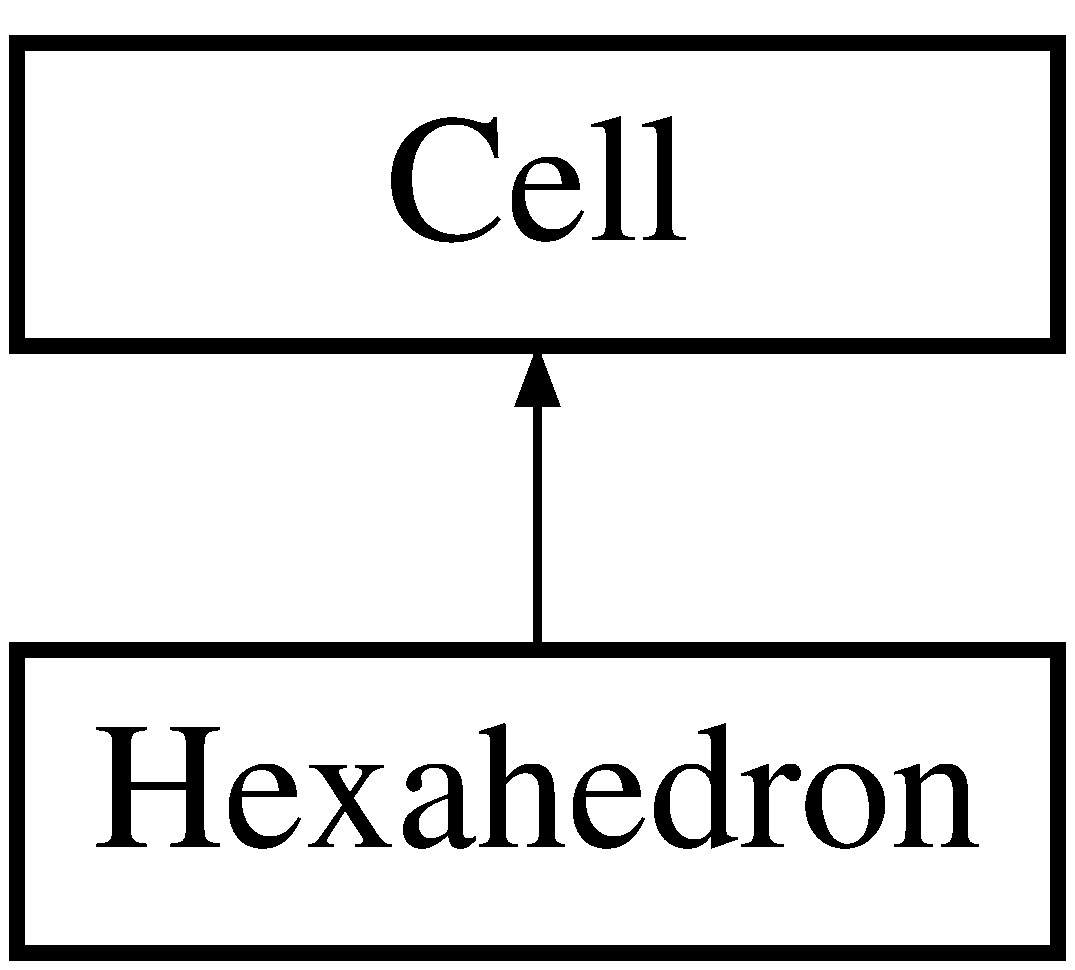
\includegraphics[height=2.000000cm]{class_hexahedron}
\end{center}
\end{figure}
\subsection*{Public Member Functions}
\begin{DoxyCompactItemize}
\item 
{\bfseries Hexahedron} (int, int, int, std\+::vector$<$ int $>$, std\+::vector$<$ \hyperlink{class_vector3_d}{Vector3D} $>$, std\+::vector$<$ \hyperlink{class_material}{Material} $>$)\hypertarget{class_hexahedron_a6144c98029c2bb69ba56b68482a1704a}{}\label{class_hexahedron_a6144c98029c2bb69ba56b68482a1704a}

\item 
{\bfseries Hexahedron} (const \hyperlink{class_cell}{Cell} \&)\hypertarget{class_hexahedron_a4f076e319bb170539c46610be559823d}{}\label{class_hexahedron_a4f076e319bb170539c46610be559823d}

\item 
void {\bfseries calculate\+Volume} (std\+::vector$<$ \hyperlink{class_vector3_d}{Vector3D} $>$)\hypertarget{class_hexahedron_a7258ffb005cdc253db5de33fd2b581ce}{}\label{class_hexahedron_a7258ffb005cdc253db5de33fd2b581ce}

\end{DoxyCompactItemize}
\subsection*{Additional Inherited Members}


The documentation for this class was generated from the following files\+:\begin{DoxyCompactItemize}
\item 
/home/travis/build/\+Te\+Fka/2020\+\_\+\+G\+R\+O\+U\+P\+\_\+19/\+Inc/Cell.\+h\item 
/home/travis/build/\+Te\+Fka/2020\+\_\+\+G\+R\+O\+U\+P\+\_\+19/\+Src/Cell.\+cpp\end{DoxyCompactItemize}

\hypertarget{class_main_window}{}\section{Main\+Window Class Reference}
\label{class_main_window}\index{Main\+Window@{Main\+Window}}
Inheritance diagram for Main\+Window\+:\begin{figure}[H]
\begin{center}
\leavevmode
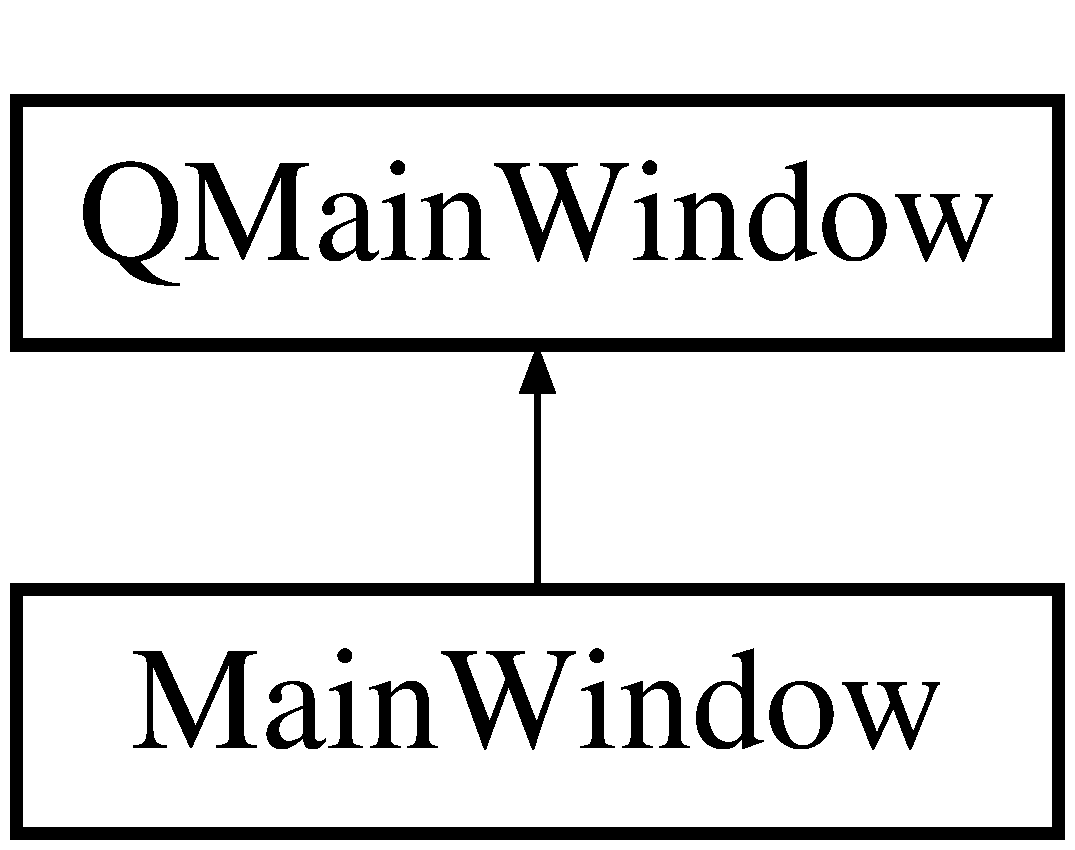
\includegraphics[height=2.000000cm]{class_main_window}
\end{center}
\end{figure}
\subsection*{Public Slots}
\begin{DoxyCompactItemize}
\item 
void {\bfseries handle\+Update} ()\hypertarget{class_main_window_a5c6cea005b60afcc4e0555e40e280e1d}{}\label{class_main_window_a5c6cea005b60afcc4e0555e40e280e1d}

\item 
void {\bfseries change\+Clip\+Value} (int)\hypertarget{class_main_window_a49b774e1f63554608bcc44d90eba8ce2}{}\label{class_main_window_a49b774e1f63554608bcc44d90eba8ce2}

\item 
void {\bfseries handle\+Open\+Button} ()\hypertarget{class_main_window_a16434089bdb53bc4c867c558c0a7fbb4}{}\label{class_main_window_a16434089bdb53bc4c867c558c0a7fbb4}

\item 
void {\bfseries handle\+Save\+Button} ()\hypertarget{class_main_window_ac52b63ed01bbdd8fd4425be619927c8a}{}\label{class_main_window_ac52b63ed01bbdd8fd4425be619927c8a}

\item 
void {\bfseries handle\+Help\+Button} ()\hypertarget{class_main_window_a919e75cfef556ae0b5611d6655734d1a}{}\label{class_main_window_a919e75cfef556ae0b5611d6655734d1a}

\item 
void {\bfseries handle\+New\+Button} ()\hypertarget{class_main_window_ab015df9a44e44eed7dfb685bd2c38295}{}\label{class_main_window_ab015df9a44e44eed7dfb685bd2c38295}

\item 
void {\bfseries set\+Camera\+Orientation\+PosX} ()\hypertarget{class_main_window_a1983dc5e6d5ccdf46e9f7d1a88835d3d}{}\label{class_main_window_a1983dc5e6d5ccdf46e9f7d1a88835d3d}

\item 
void {\bfseries set\+Camera\+Orientation\+NegX} ()\hypertarget{class_main_window_a4d572113ca36123c0c7dc765b289b413}{}\label{class_main_window_a4d572113ca36123c0c7dc765b289b413}

\item 
void {\bfseries set\+Camera\+Orientation\+PosY} ()\hypertarget{class_main_window_a4980ce0a94fd49b25bf3d005bfaf4756}{}\label{class_main_window_a4980ce0a94fd49b25bf3d005bfaf4756}

\item 
void {\bfseries set\+Camera\+Orientation\+NegY} ()\hypertarget{class_main_window_a50b850ca17eb434ff702ea5e87b3cbfe}{}\label{class_main_window_a50b850ca17eb434ff702ea5e87b3cbfe}

\item 
void {\bfseries set\+Camera\+Orientation\+PosZ} ()\hypertarget{class_main_window_aa92b6d33b290f0be1c74d83bf2c20d20}{}\label{class_main_window_aa92b6d33b290f0be1c74d83bf2c20d20}

\item 
void {\bfseries set\+Camera\+Orientation\+NegZ} ()\hypertarget{class_main_window_a867a99f44d3f38b0fc273bb914123c5d}{}\label{class_main_window_a867a99f44d3f38b0fc273bb914123c5d}

\item 
void {\bfseries set\+Camera\+Orientation\+Pos\+Shift} ()\hypertarget{class_main_window_a9419db2007e9cb2fce7c47bad9a1e24d}{}\label{class_main_window_a9419db2007e9cb2fce7c47bad9a1e24d}

\item 
void {\bfseries set\+Camera\+Orientation\+Neg\+Shift} ()\hypertarget{class_main_window_a662365afb1e72acc14a3395454af2e53}{}\label{class_main_window_a662365afb1e72acc14a3395454af2e53}

\item 
void {\bfseries set\+Camera\+Orientation\+Pos\+Rotate} ()\hypertarget{class_main_window_a337c399d18112efcaaef73894041bbb7}{}\label{class_main_window_a337c399d18112efcaaef73894041bbb7}

\item 
void {\bfseries set\+Camera\+Orientation\+Neg\+Rotate} ()\hypertarget{class_main_window_a9aa0b2b560852435780f75c2b3f10f1f}{}\label{class_main_window_a9aa0b2b560852435780f75c2b3f10f1f}

\item 
void {\bfseries reset\+Viewer} ()\hypertarget{class_main_window_aad7276b3a2f667c813d8b4d00a6995d3}{}\label{class_main_window_aad7276b3a2f667c813d8b4d00a6995d3}

\item 
void {\bfseries reset\+Camera} ()\hypertarget{class_main_window_acdfade55a70d7cba0ba0dbea3d77d183}{}\label{class_main_window_acdfade55a70d7cba0ba0dbea3d77d183}

\item 
void {\bfseries change\+Background\+Color} ()\hypertarget{class_main_window_a1a7e2b9194e7134bca5fcf1dd4842a07}{}\label{class_main_window_a1a7e2b9194e7134bca5fcf1dd4842a07}

\item 
void {\bfseries change\+Object\+Color} ()\hypertarget{class_main_window_a8f203aed440e1d68f244dec9f45cfadc}{}\label{class_main_window_a8f203aed440e1d68f244dec9f45cfadc}

\item 
void {\bfseries reset\+Object\+Color} ()\hypertarget{class_main_window_a17bfb1a5680150f099064be820b950a8}{}\label{class_main_window_a17bfb1a5680150f099064be820b950a8}

\end{DoxyCompactItemize}
\subsection*{Signals}
\begin{DoxyCompactItemize}
\item 
void {\bfseries status\+Update\+Message} (const Q\+String \&message, int timeout)\hypertarget{class_main_window_a86443ea744fda3e9bad328c2fd1c3d6b}{}\label{class_main_window_a86443ea744fda3e9bad328c2fd1c3d6b}

\end{DoxyCompactItemize}
\subsection*{Public Member Functions}
\begin{DoxyCompactItemize}
\item 
{\bfseries Main\+Window} (Q\+Widget $\ast$parent=0)\hypertarget{class_main_window_a8b244be8b7b7db1b08de2a2acb9409db}{}\label{class_main_window_a8b244be8b7b7db1b08de2a2acb9409db}

\end{DoxyCompactItemize}


The documentation for this class was generated from the following files\+:\begin{DoxyCompactItemize}
\item 
/home/travis/build/\+Te\+Fka/2020\+\_\+\+G\+R\+O\+U\+P\+\_\+19/\+G\+U\+I\+\_\+source/mainwindow.\+h\item 
/home/travis/build/\+Te\+Fka/2020\+\_\+\+G\+R\+O\+U\+P\+\_\+19/\+G\+U\+I\+\_\+source/mainwindow.\+cpp\end{DoxyCompactItemize}

\hypertarget{class_material}{}\section{Material Class Reference}
\label{class_material}\index{Material@{Material}}
\subsection*{Public Member Functions}
\begin{DoxyCompactItemize}
\item 
{\bfseries Material} (int, double, std\+::string, \hyperlink{class_vector3_d}{Vector3D})\hypertarget{class_material_adbb4e5a1a288f3a8b01296b620bbecd3}{}\label{class_material_adbb4e5a1a288f3a8b01296b620bbecd3}

\item 
int {\bfseries get\+ID} ()\hypertarget{class_material_ad31f04334fa5bc9ff16170149f037f2a}{}\label{class_material_ad31f04334fa5bc9ff16170149f037f2a}

\item 
std\+::string {\bfseries get\+Name} ()\hypertarget{class_material_a6dd6278a55af611612d999c7d3ab63f3}{}\label{class_material_a6dd6278a55af611612d999c7d3ab63f3}

\item 
double {\bfseries get\+Density} ()\hypertarget{class_material_a3601b084de60ca17f7deda89567a2a7f}{}\label{class_material_a3601b084de60ca17f7deda89567a2a7f}

\item 
\hyperlink{class_vector3_d}{Vector3D} {\bfseries get\+Color} ()\hypertarget{class_material_acf6f174b41cddbe6d8f21d11525f6f7b}{}\label{class_material_acf6f174b41cddbe6d8f21d11525f6f7b}

\item 
void {\bfseries set\+ID} (int)\hypertarget{class_material_a219ae8a9fd2ff596d28625cfb8b2b317}{}\label{class_material_a219ae8a9fd2ff596d28625cfb8b2b317}

\item 
void {\bfseries set\+Name} (std\+::string)\hypertarget{class_material_a0a0580361765d0f3c21df7f21af7981c}{}\label{class_material_a0a0580361765d0f3c21df7f21af7981c}

\item 
void {\bfseries set\+Color} (\hyperlink{class_vector3_d}{Vector3D})\hypertarget{class_material_afa395703d77b04187d6373ad330824d9}{}\label{class_material_afa395703d77b04187d6373ad330824d9}

\item 
void {\bfseries set\+Density} (double)\hypertarget{class_material_afd9ed546e6a1b4ea948f331a455fe3b6}{}\label{class_material_afd9ed546e6a1b4ea948f331a455fe3b6}

\item 
{\bfseries Material} (const \hyperlink{class_material}{Material} \&m)\hypertarget{class_material_a65005757f3572b988460eff5544e9527}{}\label{class_material_a65005757f3572b988460eff5544e9527}

\end{DoxyCompactItemize}


The documentation for this class was generated from the following files\+:\begin{DoxyCompactItemize}
\item 
/home/travis/build/\+Te\+Fka/2020\+\_\+\+G\+R\+O\+U\+P\+\_\+19/\+Inc/Material.\+h\item 
/home/travis/build/\+Te\+Fka/2020\+\_\+\+G\+R\+O\+U\+P\+\_\+19/\+Src/Material.\+cpp\end{DoxyCompactItemize}

\hypertarget{class_matrix3x3}{}\section{Matrix3x3 Class Reference}
\label{class_matrix3x3}\index{Matrix3x3@{Matrix3x3}}
\subsection*{Public Member Functions}
\begin{DoxyCompactItemize}
\item 
{\bfseries Matrix3x3} (double)\hypertarget{class_matrix3x3_a70ca799597247a19e8285f883c539366}{}\label{class_matrix3x3_a70ca799597247a19e8285f883c539366}

\item 
{\bfseries Matrix3x3} (const \hyperlink{class_matrix3x3}{Matrix3x3} \&)\hypertarget{class_matrix3x3_a1604c4113e3173740aaf284d4a798b92}{}\label{class_matrix3x3_a1604c4113e3173740aaf284d4a798b92}

\item 
double {\bfseries operator()} (int, int)\hypertarget{class_matrix3x3_a93eb28c963637058fd3da9201e93cea8}{}\label{class_matrix3x3_a93eb28c963637058fd3da9201e93cea8}

\item 
\hyperlink{class_matrix3x3}{Matrix3x3} {\bfseries operator+} (\hyperlink{class_matrix3x3}{Matrix3x3} \&)\hypertarget{class_matrix3x3_a458cb354acf25d9f4dd0f038afd48a6b}{}\label{class_matrix3x3_a458cb354acf25d9f4dd0f038afd48a6b}

\item 
\hyperlink{class_matrix3x3}{Matrix3x3} {\bfseries operator-\/} (\hyperlink{class_matrix3x3}{Matrix3x3} \&)\hypertarget{class_matrix3x3_ad6097601c5d9779505cc1bb96a53fd8a}{}\label{class_matrix3x3_ad6097601c5d9779505cc1bb96a53fd8a}

\item 
\hyperlink{class_matrix3x3}{Matrix3x3} {\bfseries operator$\ast$} (\hyperlink{class_matrix3x3}{Matrix3x3} \&)\hypertarget{class_matrix3x3_ac973064b3cd3d4115e719a7eec3e4ae3}{}\label{class_matrix3x3_ac973064b3cd3d4115e719a7eec3e4ae3}

\item 
\hyperlink{class_vector3_d}{Vector3D} {\bfseries operator$\ast$} (\hyperlink{class_vector3_d}{Vector3D} \&)\hypertarget{class_matrix3x3_a754dc9a5e7c88d6d4d00f028f248d77a}{}\label{class_matrix3x3_a754dc9a5e7c88d6d4d00f028f248d77a}

\item 
void {\bfseries set\+Value} (int, int, double)\hypertarget{class_matrix3x3_a139eaa4d6a29aee712456f2156367406}{}\label{class_matrix3x3_a139eaa4d6a29aee712456f2156367406}

\item 
std\+::vector$<$ std\+::vector$<$ double $>$ $>$ {\bfseries get\+Matrix3x3} ()\hypertarget{class_matrix3x3_a8f22384da78b154f454241659b731466}{}\label{class_matrix3x3_a8f22384da78b154f454241659b731466}

\item 
void {\bfseries set\+Identity\+Matrix3x3} ()\hypertarget{class_matrix3x3_ad3aec636b7f82d5874c94f7b70b9cd1b}{}\label{class_matrix3x3_ad3aec636b7f82d5874c94f7b70b9cd1b}

\item 
void {\bfseries invert} ()\hypertarget{class_matrix3x3_aed02f0e19f32d1f633483f91c48e6538}{}\label{class_matrix3x3_aed02f0e19f32d1f633483f91c48e6538}

\item 
void {\bfseries transpose} ()\hypertarget{class_matrix3x3_a17970c50970d868be9657283e7d7912b}{}\label{class_matrix3x3_a17970c50970d868be9657283e7d7912b}

\item 
\hyperlink{class_matrix3x3}{Matrix3x3} {\bfseries get\+Rotation\+Matrix3x3} (double, double, double, double)\hypertarget{class_matrix3x3_a1cacc9b5af0d31f305bf5f45b930cc3d}{}\label{class_matrix3x3_a1cacc9b5af0d31f305bf5f45b930cc3d}

\end{DoxyCompactItemize}
\subsection*{Friends}
\begin{DoxyCompactItemize}
\item 
class {\bfseries Vector3D}\hypertarget{class_matrix3x3_a166ef6ddf8d6949db83102b57b30401a}{}\label{class_matrix3x3_a166ef6ddf8d6949db83102b57b30401a}

\end{DoxyCompactItemize}


The documentation for this class was generated from the following files\+:\begin{DoxyCompactItemize}
\item 
/home/travis/build/\+Te\+Fka/2020\+\_\+\+G\+R\+O\+U\+P\+\_\+19/\+Inc/Matrix3x3.\+h\item 
/home/travis/build/\+Te\+Fka/2020\+\_\+\+G\+R\+O\+U\+P\+\_\+19/\+Src/Matrix3x3.\+cpp\end{DoxyCompactItemize}

\hypertarget{class_model}{}\section{Model Class Reference}
\label{class_model}\index{Model@{Model}}
\subsection*{Public Member Functions}
\begin{DoxyCompactItemize}
\item 
{\bfseries Model} (char $\ast$)\hypertarget{class_model_acf455b46c4e80f1736f0d81b67bea1f8}{}\label{class_model_acf455b46c4e80f1736f0d81b67bea1f8}

\item 
{\bfseries Model} (const \hyperlink{class_model}{Model} \&)\hypertarget{class_model_a0386968ae522e868e3b6028c8b154837}{}\label{class_model_a0386968ae522e868e3b6028c8b154837}

\item 
bool {\bfseries load\+Model} (const char $\ast$)\hypertarget{class_model_a25792de725bf3e5d16b6d17af762f49a}{}\label{class_model_a25792de725bf3e5d16b6d17af762f49a}

\item 
void {\bfseries calc\+Model\+Center} ()\hypertarget{class_model_a554d27aa6a6d2e93be7d957f3b610f78}{}\label{class_model_a554d27aa6a6d2e93be7d957f3b610f78}

\item 
\hyperlink{class_vector3_d}{Vector3D} {\bfseries get\+Model\+Center} ()\hypertarget{class_model_a3616941d01a129c90a81891f6aa78819}{}\label{class_model_a3616941d01a129c90a81891f6aa78819}

\item 
\hyperlink{class_vector3_d}{Vector3D} {\bfseries get\+Model\+Dimensions} ()\hypertarget{class_model_a11ca5f07bd3e8b60ed5cb70ab673dc50}{}\label{class_model_a11ca5f07bd3e8b60ed5cb70ab673dc50}

\item 
std\+::vector$<$ \hyperlink{class_vector3_d}{Vector3D} $>$ {\bfseries get\+Vectors} ()\hypertarget{class_model_ab37cfe36bfc8ba85a0894cb11c156e11}{}\label{class_model_ab37cfe36bfc8ba85a0894cb11c156e11}

\item 
std\+::vector$<$ \hyperlink{class_material}{Material} $>$ {\bfseries get\+Materials} ()\hypertarget{class_model_acebb51323259e2f11494e0626490c64e}{}\label{class_model_acebb51323259e2f11494e0626490c64e}

\item 
std\+::vector$<$ \hyperlink{class_cell}{Cell} $>$ {\bfseries get\+Cells} ()\hypertarget{class_model_af1b55cd1a07b6ecf6858c78ebc3d56d0}{}\label{class_model_af1b55cd1a07b6ecf6858c78ebc3d56d0}

\item 
\hyperlink{class_cell}{Cell} {\bfseries get\+Cell} (int)\hypertarget{class_model_a4a57497301bb2ab1d8dee7dfc1b7a240}{}\label{class_model_a4a57497301bb2ab1d8dee7dfc1b7a240}

\item 
\hyperlink{class_vector3_d}{Vector3D} {\bfseries get\+Vector} (int)\hypertarget{class_model_a6d877aa2a535c2a613fd92d6ef80b576}{}\label{class_model_a6d877aa2a535c2a613fd92d6ef80b576}

\item 
\hyperlink{class_material}{Material} {\bfseries get\+Material} (int)\hypertarget{class_model_a9dfba34e1752702d74e8c77e3f591b3f}{}\label{class_model_a9dfba34e1752702d74e8c77e3f591b3f}

\item 
int {\bfseries get\+Vector\+Amount} ()\hypertarget{class_model_acd0f324509ae2321c04f259fd0133a7a}{}\label{class_model_acd0f324509ae2321c04f259fd0133a7a}

\item 
int {\bfseries get\+Cell\+Amount} ()\hypertarget{class_model_a29b97b575c9ebfa2aaa9806cfa094f1e}{}\label{class_model_a29b97b575c9ebfa2aaa9806cfa094f1e}

\item 
void {\bfseries show\+Materials} ()\hypertarget{class_model_ae7b7dfcec56ec095782b672745f64c7e}{}\label{class_model_ae7b7dfcec56ec095782b672745f64c7e}

\item 
void {\bfseries show\+Vectors} ()\hypertarget{class_model_ac6201ae8b810e878da7c0af337cc6e84}{}\label{class_model_ac6201ae8b810e878da7c0af337cc6e84}

\item 
void {\bfseries show\+Cells} ()\hypertarget{class_model_adb18726e9aee1ec6f0980f5e4624e481}{}\label{class_model_adb18726e9aee1ec6f0980f5e4624e481}

\item 
void {\bfseries load\+Info\+To\+File} (char $\ast$)\hypertarget{class_model_a6f31f2c1849ca236b837521a5303f320}{}\label{class_model_a6f31f2c1849ca236b837521a5303f320}

\end{DoxyCompactItemize}


The documentation for this class was generated from the following files\+:\begin{DoxyCompactItemize}
\item 
/home/travis/build/\+Te\+Fka/2020\+\_\+\+G\+R\+O\+U\+P\+\_\+19/\+Inc/Model.\+h\item 
/home/travis/build/\+Te\+Fka/2020\+\_\+\+G\+R\+O\+U\+P\+\_\+19/\+Src/Model.\+cpp\end{DoxyCompactItemize}

\hypertarget{class_new_shape_choice}{}\section{New\+Shape\+Choice Class Reference}
\label{class_new_shape_choice}\index{New\+Shape\+Choice@{New\+Shape\+Choice}}
Inheritance diagram for New\+Shape\+Choice\+:\begin{figure}[H]
\begin{center}
\leavevmode
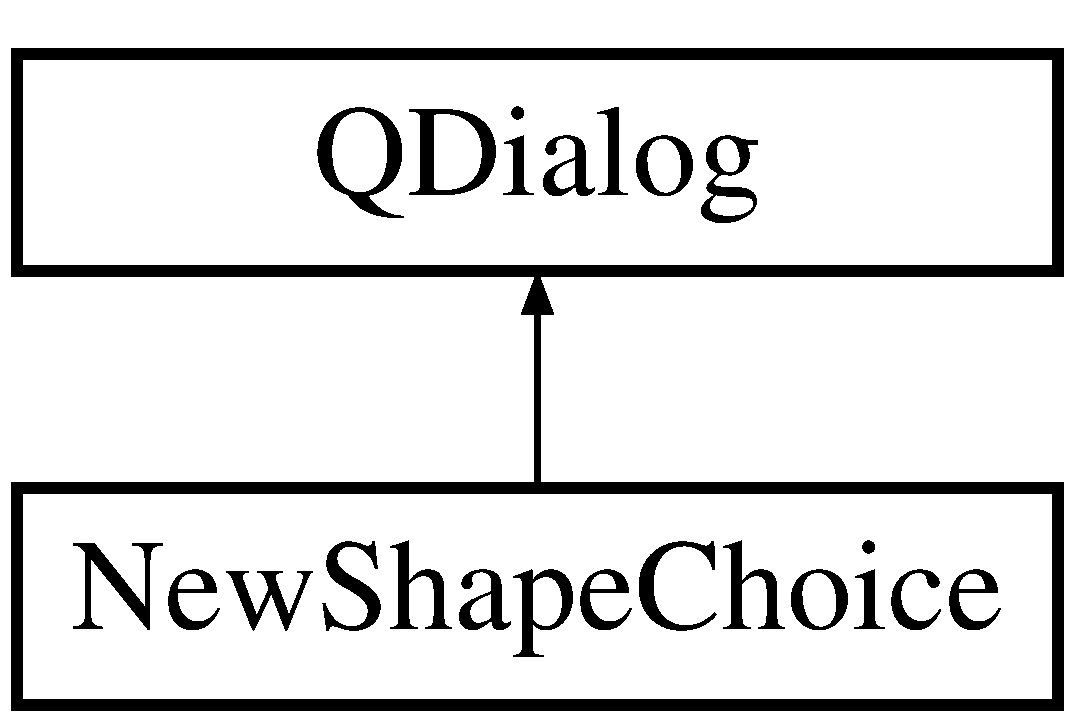
\includegraphics[height=2.000000cm]{class_new_shape_choice}
\end{center}
\end{figure}
\subsection*{Public Slots}
\begin{DoxyCompactItemize}
\item 
void {\bfseries pick\+Hexahedron} ()\hypertarget{class_new_shape_choice_adff2516ba56da550a46b029b2459f57c}{}\label{class_new_shape_choice_adff2516ba56da550a46b029b2459f57c}

\item 
void {\bfseries pick\+Tetrahedron} ()\hypertarget{class_new_shape_choice_a4df3d2e466ff4a554d2d866c751ff309}{}\label{class_new_shape_choice_a4df3d2e466ff4a554d2d866c751ff309}

\item 
void {\bfseries pick\+Pyramid} ()\hypertarget{class_new_shape_choice_a99107839c97c1d3a3e9e8782cb62af63}{}\label{class_new_shape_choice_a99107839c97c1d3a3e9e8782cb62af63}

\item 
void {\bfseries pick\+Sphere} ()\hypertarget{class_new_shape_choice_a07c2f93ed76719508c4252fdb5f4de11}{}\label{class_new_shape_choice_a07c2f93ed76719508c4252fdb5f4de11}

\item 
void {\bfseries pick\+Disk} ()\hypertarget{class_new_shape_choice_ab51c5ccbc969afb8ccfb310e3feeca3e}{}\label{class_new_shape_choice_ab51c5ccbc969afb8ccfb310e3feeca3e}

\item 
void {\bfseries pick\+Cone} ()\hypertarget{class_new_shape_choice_a71c21786d9831dab8f2d1bf7513b5c4e}{}\label{class_new_shape_choice_a71c21786d9831dab8f2d1bf7513b5c4e}

\item 
void {\bfseries pick\+Plane} ()\hypertarget{class_new_shape_choice_a71dbaaceeafb7eae5860b892e6b14a56}{}\label{class_new_shape_choice_a71dbaaceeafb7eae5860b892e6b14a56}

\item 
void {\bfseries pick\+Points} ()\hypertarget{class_new_shape_choice_abce250b07adb0ce8bc2b13939e9d130e}{}\label{class_new_shape_choice_abce250b07adb0ce8bc2b13939e9d130e}

\item 
void {\bfseries pick\+Line} ()\hypertarget{class_new_shape_choice_a2417759d30f97495b450df2333a1746c}{}\label{class_new_shape_choice_a2417759d30f97495b450df2333a1746c}

\item 
void {\bfseries pick\+Cylinder} ()\hypertarget{class_new_shape_choice_a153bf60861c5da2724890c8158b4faca}{}\label{class_new_shape_choice_a153bf60861c5da2724890c8158b4faca}

\end{DoxyCompactItemize}
\subsection*{Public Member Functions}
\begin{DoxyCompactItemize}
\item 
{\bfseries New\+Shape\+Choice} (Q\+Widget $\ast$parent=nullptr)\hypertarget{class_new_shape_choice_a8fd6fbdd0fe0ac1a250729389d656247}{}\label{class_new_shape_choice_a8fd6fbdd0fe0ac1a250729389d656247}

\item 
bool {\bfseries run\+Choice} (int \&)\hypertarget{class_new_shape_choice_a0ad3ab9d4e869400468e1f2a758e22e4}{}\label{class_new_shape_choice_a0ad3ab9d4e869400468e1f2a758e22e4}

\end{DoxyCompactItemize}


The documentation for this class was generated from the following files\+:\begin{DoxyCompactItemize}
\item 
/home/travis/build/\+Te\+Fka/2020\+\_\+\+G\+R\+O\+U\+P\+\_\+19/\+G\+U\+I\+\_\+source/newshapechoice.\+h\item 
/home/travis/build/\+Te\+Fka/2020\+\_\+\+G\+R\+O\+U\+P\+\_\+19/\+G\+U\+I\+\_\+source/newshapechoice.\+cpp\end{DoxyCompactItemize}

\hypertarget{class_pyramid}{}\section{Pyramid Class Reference}
\label{class_pyramid}\index{Pyramid@{Pyramid}}
Inheritance diagram for Pyramid\+:\begin{figure}[H]
\begin{center}
\leavevmode
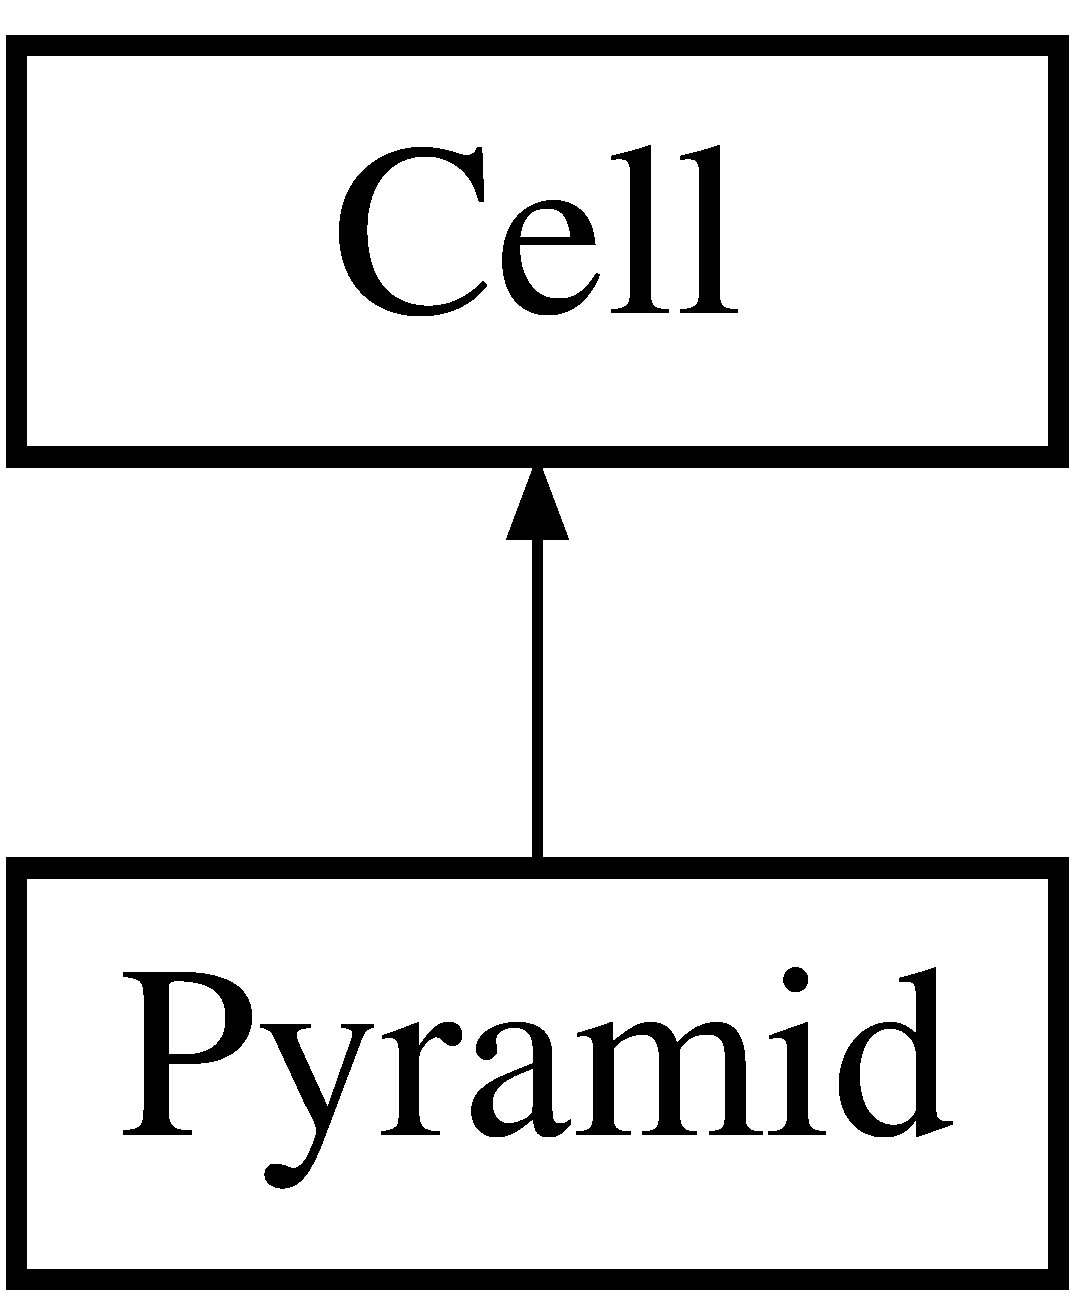
\includegraphics[height=2.000000cm]{class_pyramid}
\end{center}
\end{figure}
\subsection*{Public Member Functions}
\begin{DoxyCompactItemize}
\item 
{\bfseries Pyramid} (int, int, int, std\+::vector$<$ int $>$, std\+::vector$<$ \hyperlink{class_vector3_d}{Vector3D} $>$, std\+::vector$<$ \hyperlink{class_material}{Material} $>$)\hypertarget{class_pyramid_a2bf002316570b7e3b9b28c302b0d0259}{}\label{class_pyramid_a2bf002316570b7e3b9b28c302b0d0259}

\item 
{\bfseries Pyramid} (const \hyperlink{class_cell}{Cell} \&)\hypertarget{class_pyramid_aea1431df57752208f06d9f0e3d1bcb3b}{}\label{class_pyramid_aea1431df57752208f06d9f0e3d1bcb3b}

\item 
void {\bfseries calculate\+Volume} (std\+::vector$<$ \hyperlink{class_vector3_d}{Vector3D} $>$)\hypertarget{class_pyramid_a618910cb445a8b22d784905fda2ec2bc}{}\label{class_pyramid_a618910cb445a8b22d784905fda2ec2bc}

\end{DoxyCompactItemize}
\subsection*{Additional Inherited Members}


The documentation for this class was generated from the following files\+:\begin{DoxyCompactItemize}
\item 
/home/travis/build/\+Te\+Fka/2020\+\_\+\+G\+R\+O\+U\+P\+\_\+19/\+Inc/Cell.\+h\item 
/home/travis/build/\+Te\+Fka/2020\+\_\+\+G\+R\+O\+U\+P\+\_\+19/\+Src/Cell.\+cpp\end{DoxyCompactItemize}

\hypertarget{class_tetrahedron}{}\section{Tetrahedron Class Reference}
\label{class_tetrahedron}\index{Tetrahedron@{Tetrahedron}}
Inheritance diagram for Tetrahedron\+:\begin{figure}[H]
\begin{center}
\leavevmode
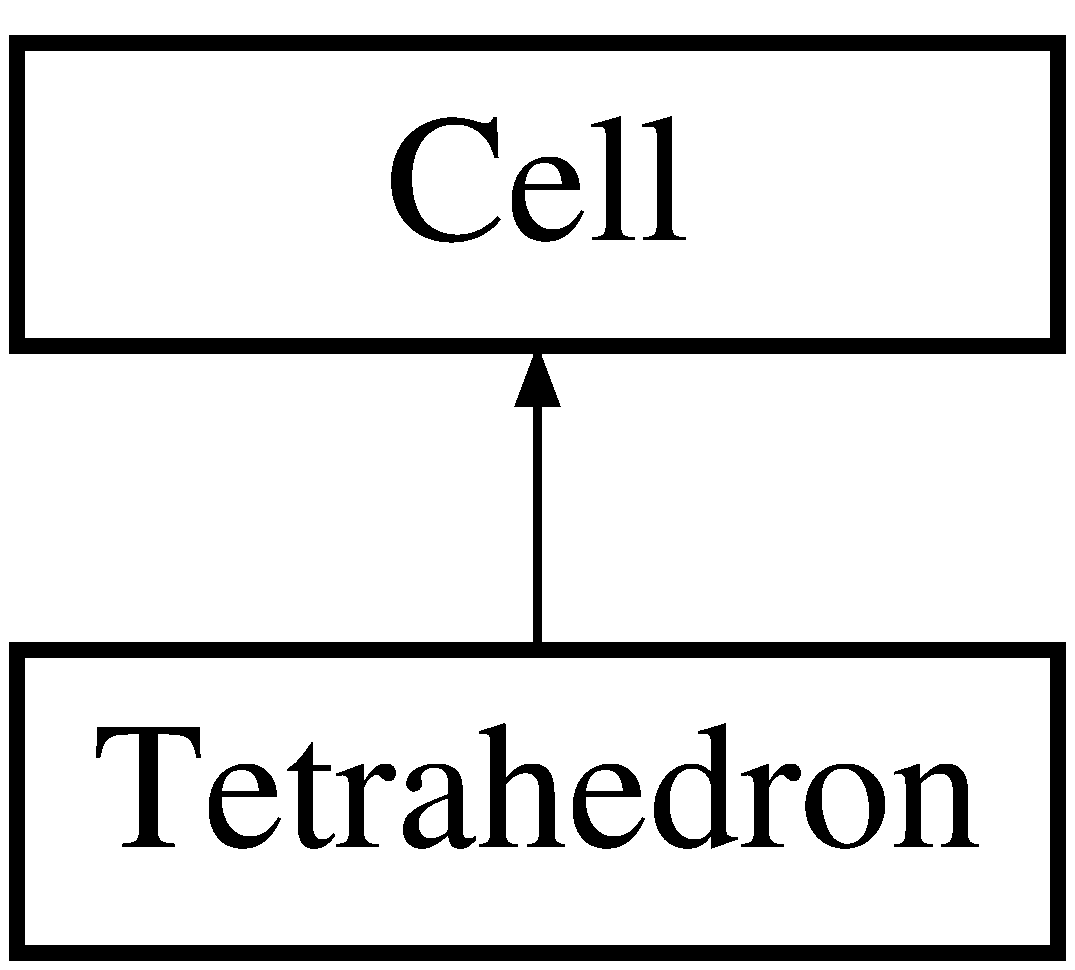
\includegraphics[height=2.000000cm]{class_tetrahedron}
\end{center}
\end{figure}
\subsection*{Public Member Functions}
\begin{DoxyCompactItemize}
\item 
{\bfseries Tetrahedron} (int, int, int, std\+::vector$<$ int $>$, std\+::vector$<$ \hyperlink{class_vector3_d}{Vector3D} $>$, std\+::vector$<$ \hyperlink{class_material}{Material} $>$)\hypertarget{class_tetrahedron_ab98a7c969ce1346e669d9ddf50130277}{}\label{class_tetrahedron_ab98a7c969ce1346e669d9ddf50130277}

\item 
{\bfseries Tetrahedron} (const \hyperlink{class_cell}{Cell} \&)\hypertarget{class_tetrahedron_a5354ba6af7ce91ffbc4a5b84df470bd7}{}\label{class_tetrahedron_a5354ba6af7ce91ffbc4a5b84df470bd7}

\item 
void {\bfseries calculate\+Volume} (std\+::vector$<$ \hyperlink{class_vector3_d}{Vector3D} $>$)\hypertarget{class_tetrahedron_a9774470bf91e164e3d8c589a9ec95857}{}\label{class_tetrahedron_a9774470bf91e164e3d8c589a9ec95857}

\end{DoxyCompactItemize}
\subsection*{Additional Inherited Members}


The documentation for this class was generated from the following files\+:\begin{DoxyCompactItemize}
\item 
/home/travis/build/\+Te\+Fka/2020\+\_\+\+G\+R\+O\+U\+P\+\_\+19/\+Inc/Cell.\+h\item 
/home/travis/build/\+Te\+Fka/2020\+\_\+\+G\+R\+O\+U\+P\+\_\+19/\+Src/Cell.\+cpp\end{DoxyCompactItemize}

\hypertarget{class_vector3_d}{}\section{Vector3D Class Reference}
\label{class_vector3_d}\index{Vector3D@{Vector3D}}
\subsection*{Public Member Functions}
\begin{DoxyCompactItemize}
\item 
{\bfseries Vector3D} (double, double, double)\hypertarget{class_vector3_d_a46f27d7bc47396e866b1921d315af059}{}\label{class_vector3_d_a46f27d7bc47396e866b1921d315af059}

\item 
{\bfseries Vector3D} (const \hyperlink{class_vector3_d}{Vector3D} \&vec)\hypertarget{class_vector3_d_a633baeac49ac713d9ae4cdf061ee9ecf}{}\label{class_vector3_d_a633baeac49ac713d9ae4cdf061ee9ecf}

\item 
void {\bfseries set\+ID} (int)\hypertarget{class_vector3_d_aa0da3e0a1eaee2afab055f0ee1b81890}{}\label{class_vector3_d_aa0da3e0a1eaee2afab055f0ee1b81890}

\item 
void {\bfseries setx} (double)\hypertarget{class_vector3_d_a75b4ba79d772f9a3fc9279c42e825dde}{}\label{class_vector3_d_a75b4ba79d772f9a3fc9279c42e825dde}

\item 
void {\bfseries sety} (double)\hypertarget{class_vector3_d_a491df193924ad7d506118d3c2107e534}{}\label{class_vector3_d_a491df193924ad7d506118d3c2107e534}

\item 
void {\bfseries setz} (double)\hypertarget{class_vector3_d_a677b550d243c23199a3770ee81153464}{}\label{class_vector3_d_a677b550d243c23199a3770ee81153464}

\item 
int {\bfseries get\+ID} ()\hypertarget{class_vector3_d_ae1417b327719d8976fbeb043a133731d}{}\label{class_vector3_d_ae1417b327719d8976fbeb043a133731d}

\item 
double {\bfseries getx} ()\hypertarget{class_vector3_d_a15c82882374b06215f64f0e7329a23db}{}\label{class_vector3_d_a15c82882374b06215f64f0e7329a23db}

\item 
double {\bfseries gety} ()\hypertarget{class_vector3_d_a891207bd6706565ae15443379d772565}{}\label{class_vector3_d_a891207bd6706565ae15443379d772565}

\item 
double {\bfseries getz} ()\hypertarget{class_vector3_d_ab69939399a0e1d5b438d7ce0bfc7b0a0}{}\label{class_vector3_d_ab69939399a0e1d5b438d7ce0bfc7b0a0}

\item 
\hyperlink{class_vector3_d}{Vector3D} {\bfseries operator+} (const \hyperlink{class_vector3_d}{Vector3D} \&vec)\hypertarget{class_vector3_d_a4cd00277b6c9701aeeaab5fa7b744c26}{}\label{class_vector3_d_a4cd00277b6c9701aeeaab5fa7b744c26}

\item 
\hyperlink{class_vector3_d}{Vector3D} {\bfseries operator-\/} (const \hyperlink{class_vector3_d}{Vector3D} \&vec)\hypertarget{class_vector3_d_ac61ff2094b3f508af31eed2e2c51136d}{}\label{class_vector3_d_ac61ff2094b3f508af31eed2e2c51136d}

\item 
double {\bfseries operator$\ast$} (const \hyperlink{class_vector3_d}{Vector3D} \&vec)\hypertarget{class_vector3_d_a092e054a30060ab9d95cf1c8a9121e2a}{}\label{class_vector3_d_a092e054a30060ab9d95cf1c8a9121e2a}

\item 
\hyperlink{class_vector3_d}{Vector3D} {\bfseries cross\+\_\+product} (const \hyperlink{class_vector3_d}{Vector3D} \&vec)\hypertarget{class_vector3_d_a9788b8a0f2deeb37bee08a6df7b1e94d}{}\label{class_vector3_d_a9788b8a0f2deeb37bee08a6df7b1e94d}

\end{DoxyCompactItemize}


The documentation for this class was generated from the following files\+:\begin{DoxyCompactItemize}
\item 
/home/travis/build/\+Te\+Fka/2020\+\_\+\+G\+R\+O\+U\+P\+\_\+19/\+Inc/Vector3\+D.\+h\item 
/home/travis/build/\+Te\+Fka/2020\+\_\+\+G\+R\+O\+U\+P\+\_\+19/\+Src/Vector3\+D.\+cpp\end{DoxyCompactItemize}

%--- End generated contents ---

% Index
\backmatter
\newpage
\phantomsection
\clearemptydoublepage
\addcontentsline{toc}{chapter}{Index}
\printindex

\end{document}
